\chapter{戦場の両面：日本人墓地と英連邦戦争墓地}

\section{二つの墓地、一つの島}

シンガポールは極めて小さな島だが、その狭い土地の中に、一つの戦争の両面が同時に葬られている。

一方には日本人墓地公園――都市の片隅で静かに眠り、雑草とブーゲンビリアが絡み合い、墓石は風化して年月の斑が刻まれている。もう一方には英連邦戦争記念公園（Kranji War Memorial Park）――英連邦戦争墓地委員会が資金を出して維持管理し、芝生は整然と刈り込まれ、白い墓碑が整列して厳かに立ち並ぶ。

前者に眠るのは侵略者たち、そして歴史に忘れられた女性たち。後者に眠るのは侵略された側の人々、そしてある都市の陥落の記憶だ。

\section{日本人墓地公園：時間に忘れられた場所}

日本人墓地公園はシンガポール北東部の後港（Hougang）にある。住所は 22 Chuan Hoe Ave。面積約29,000平方メートルで、910基の墓碑を持つ、東南アジア最大の日本人墓地だ。1969年、シンガポール政府は墓地の所有権を\textbf{日本人協会（Japanese Association of Singapore）}に返還し、以後その管理下に置かれている。1987年には正式に記念公園に指定された。

日本人墓地公園に入って最初に感じるのは、静寂だ。

厳粛な静寂ではなく、忘れ去られた静寂だ。墓地の石碑はほとんどが低く質素で、表面には苔が生え、傾いているものや崩れているものもある。マゼンタ色のブーゲンビリアが横から這い上がり、いくつかの墓石を覆っている――鮮やかな花の色が灰色の石碑と奇妙なコントラストを作り出す。生と死が、ここでは予想外の形で並置されている。

\begin{figure}[h]
\centering
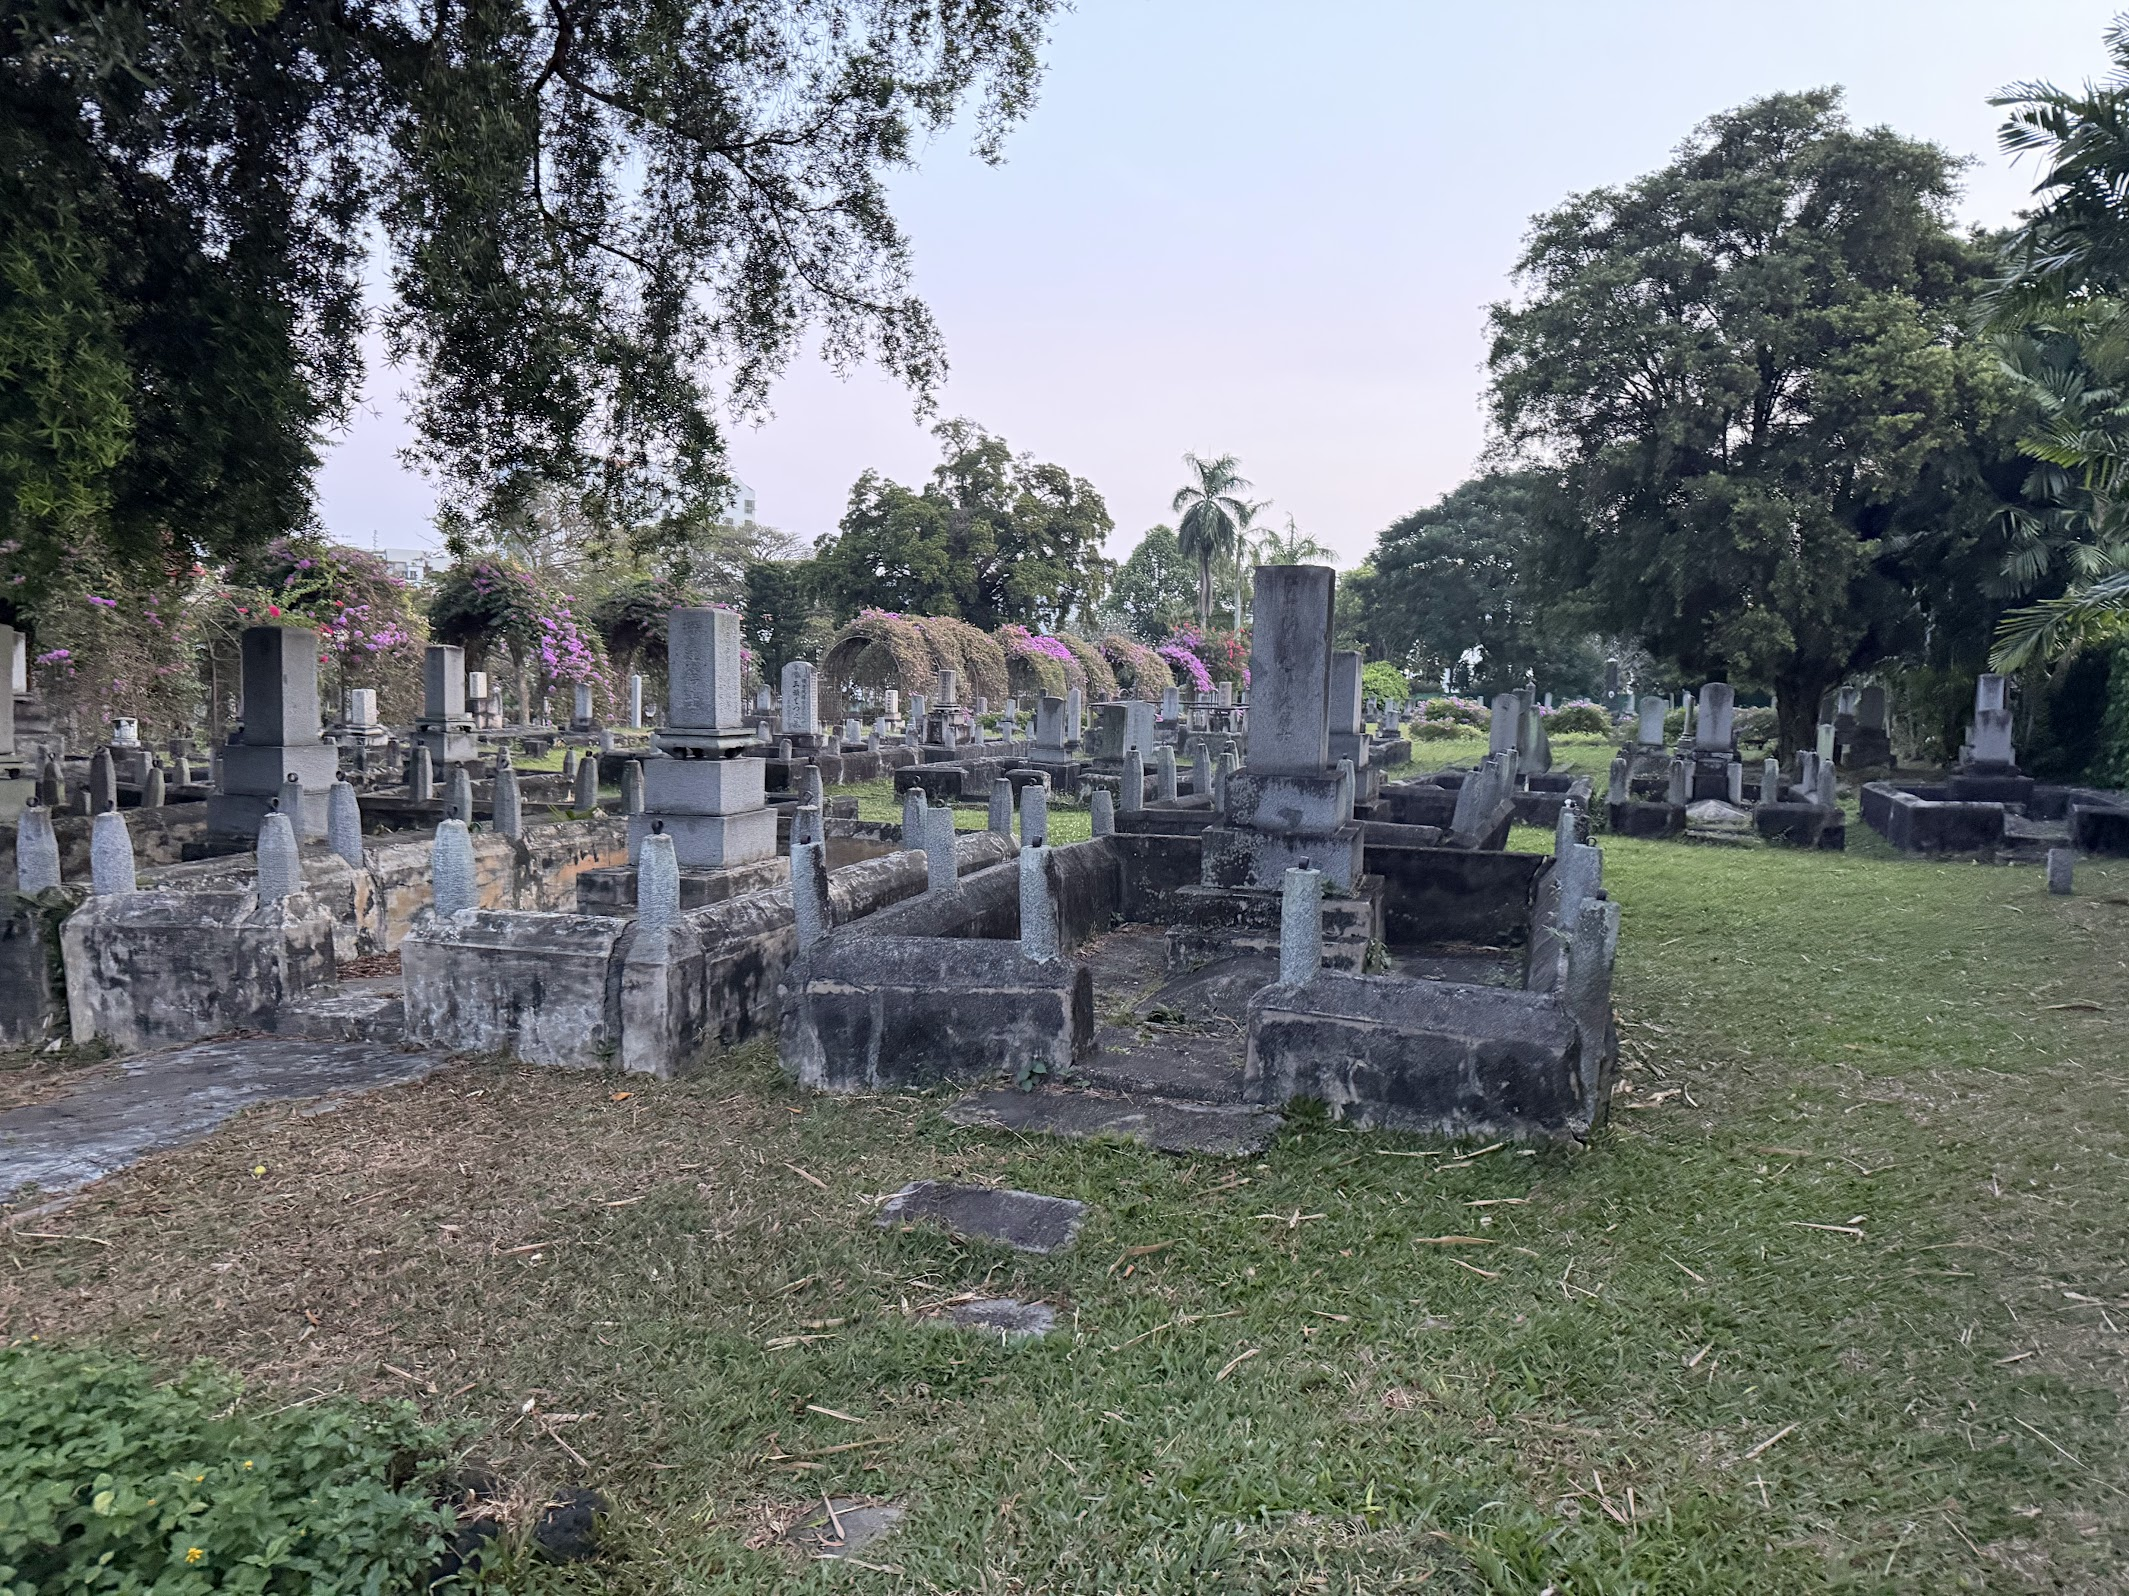
\includegraphics[width=0.8\textwidth]{../../pictures/japanese tomb/IMG_9019}
\caption{風化した墓碑に這い上がるブーゲンビリア}
\end{figure}

広い草地に数十基の墓碑が点在し、間隔は不規則で、整然とした秩序感はない。朝や夕暮れの柔らかな光が差し込むと、墓地全体がひときわ空虚に感じられる。

\begin{figure}[h]
\centering
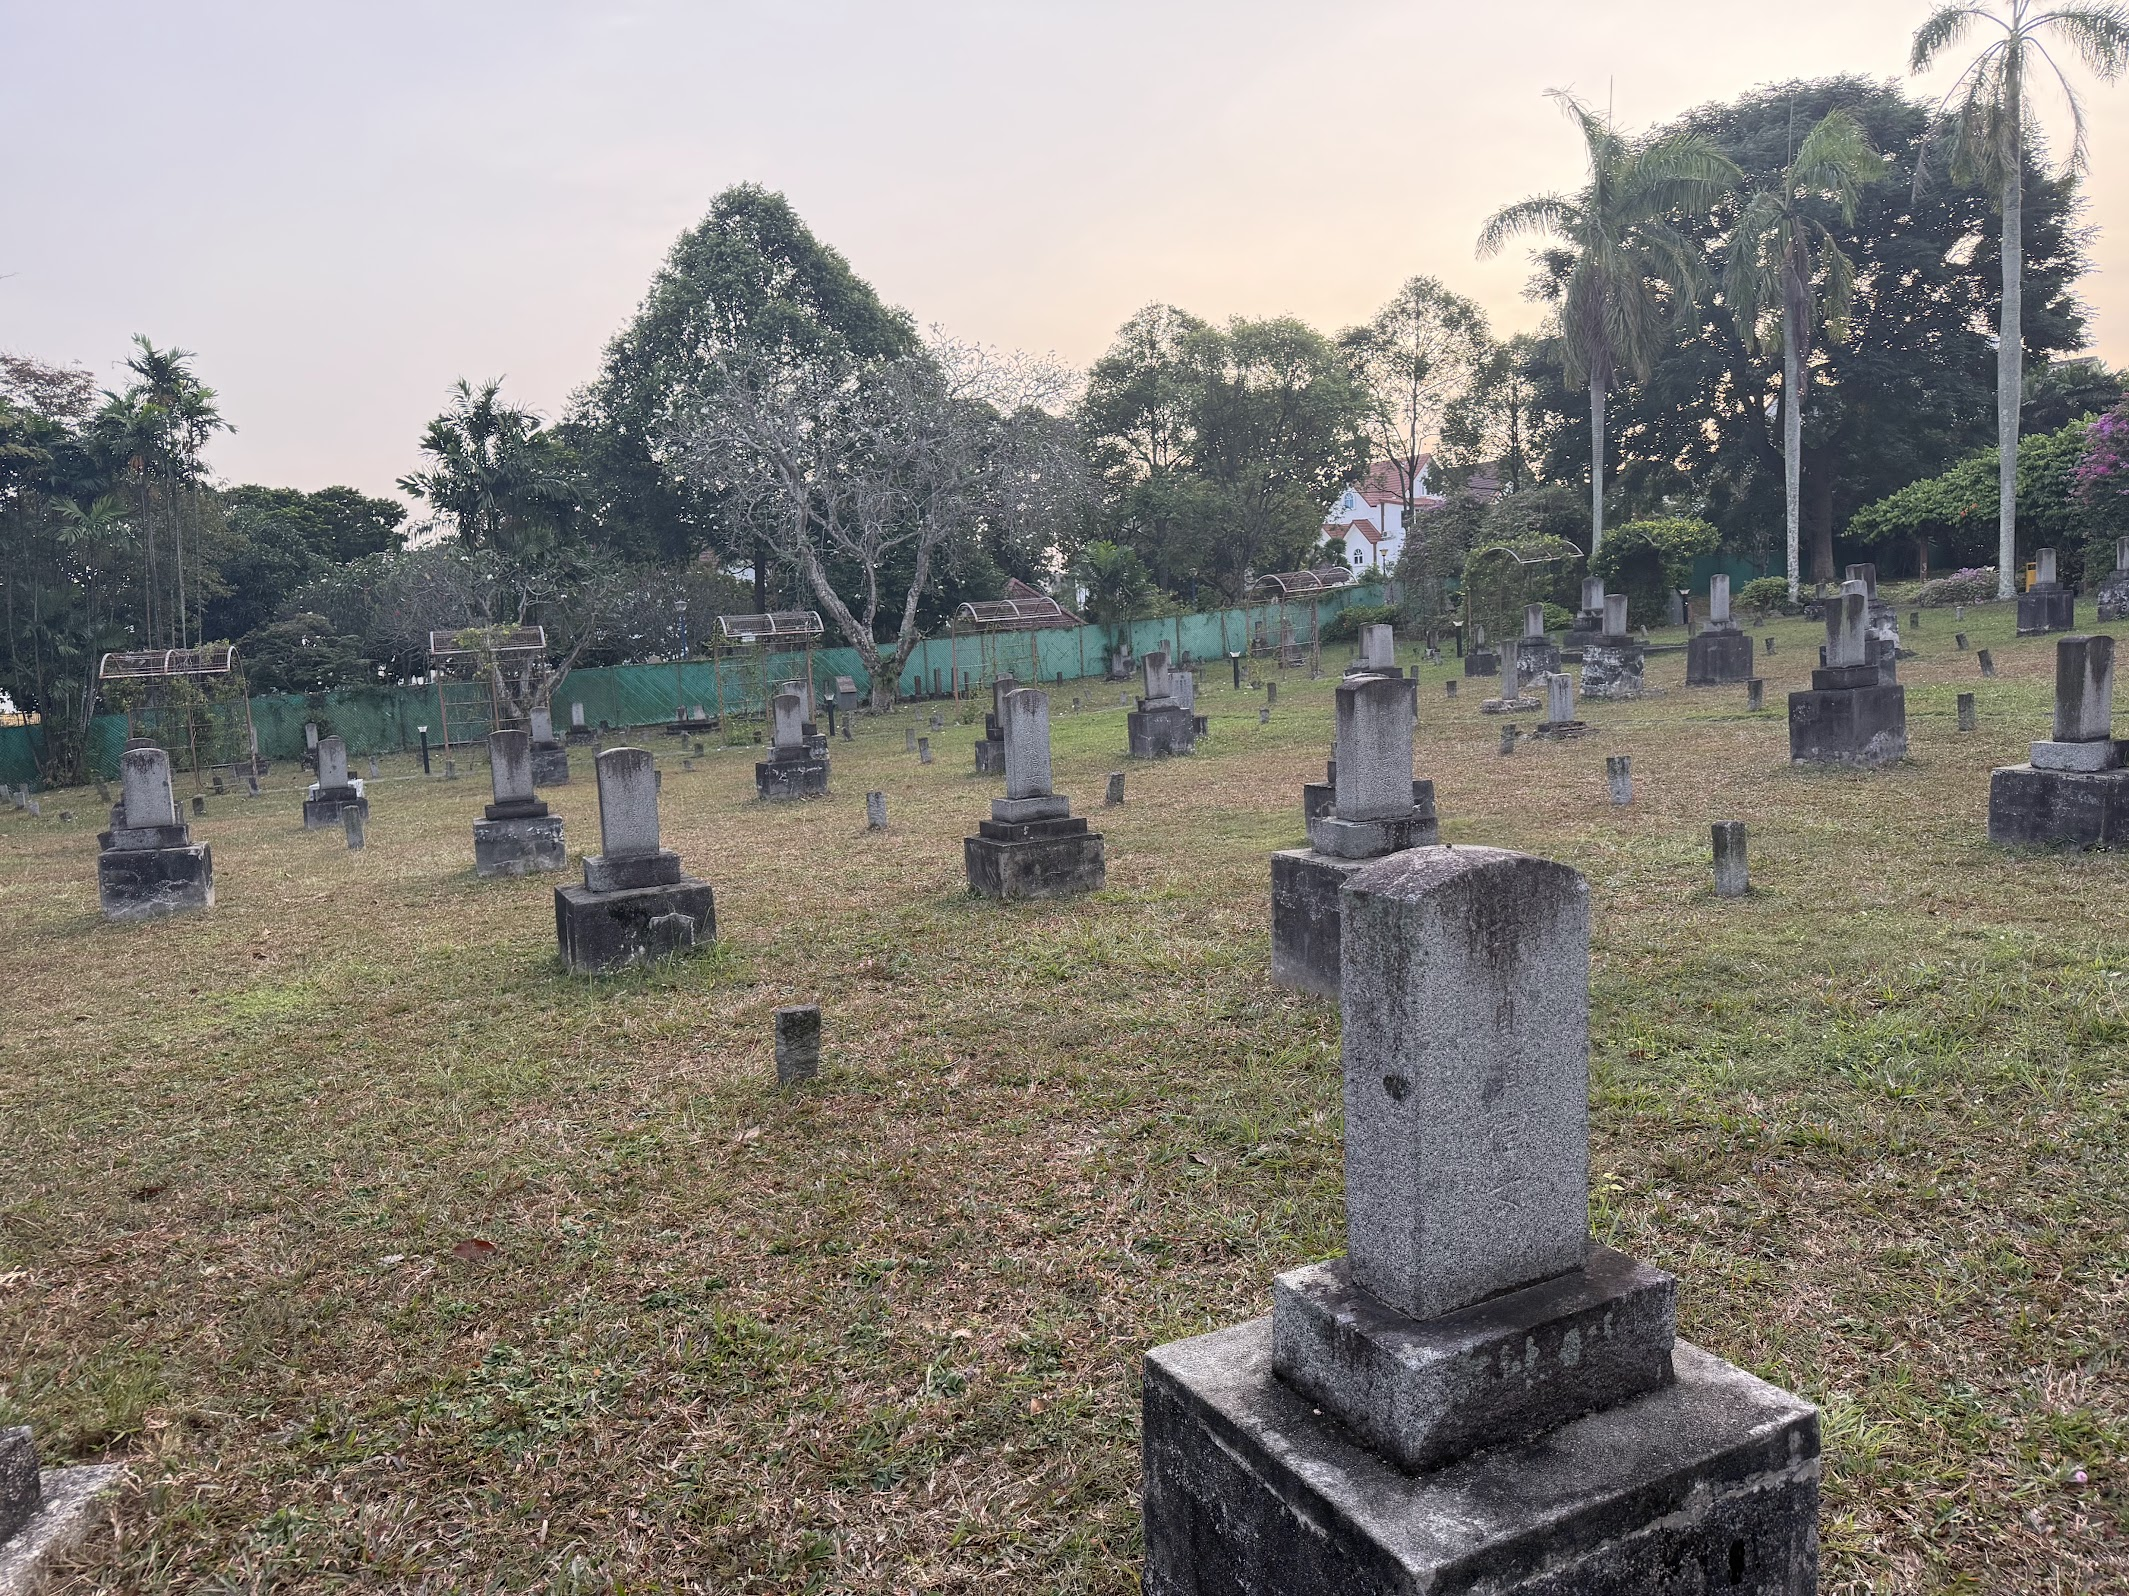
\includegraphics[width=0.8\textwidth]{../../pictures/japanese tomb/IMG_9080}
\caption{墓地全景：草地に点在する低い墓碑}
\end{figure}

\section{パイオニア墓地：名を刻まれた七十七人の女性たち}

墓地の一角に説明板がある。見出しには「先進墓地（ぱいおにあ）」――パイオニア・セメタリーとある。

説明板は\textbf{Toma Sato}という女性を紹介している。1899年没。彼女は\textbf{唐行きさん（からゆきさん）}だ――19世紀末から20世紀初頭にかけて、多くの日本人女性が東南アジアに渡り、その多くが性産業に従事した。彼女たちは「唐行きさん」と呼ばれた。「唐の国（中国）へ行った人」という意味だが、実際には東南アジア全域に足跡を残した。

説明板には、この塀の内側に\textbf{77基の墓}があり、すべて唐行きさんのもので、没年は\textbf{1899年から1938年}にわたると記されている。この墓地はかつてイギリス植民地政府に土地の境界標識として使われた――彼女たちは死後も、植民地の地図の座標となったのだ。

\begin{figure}[h]
\centering
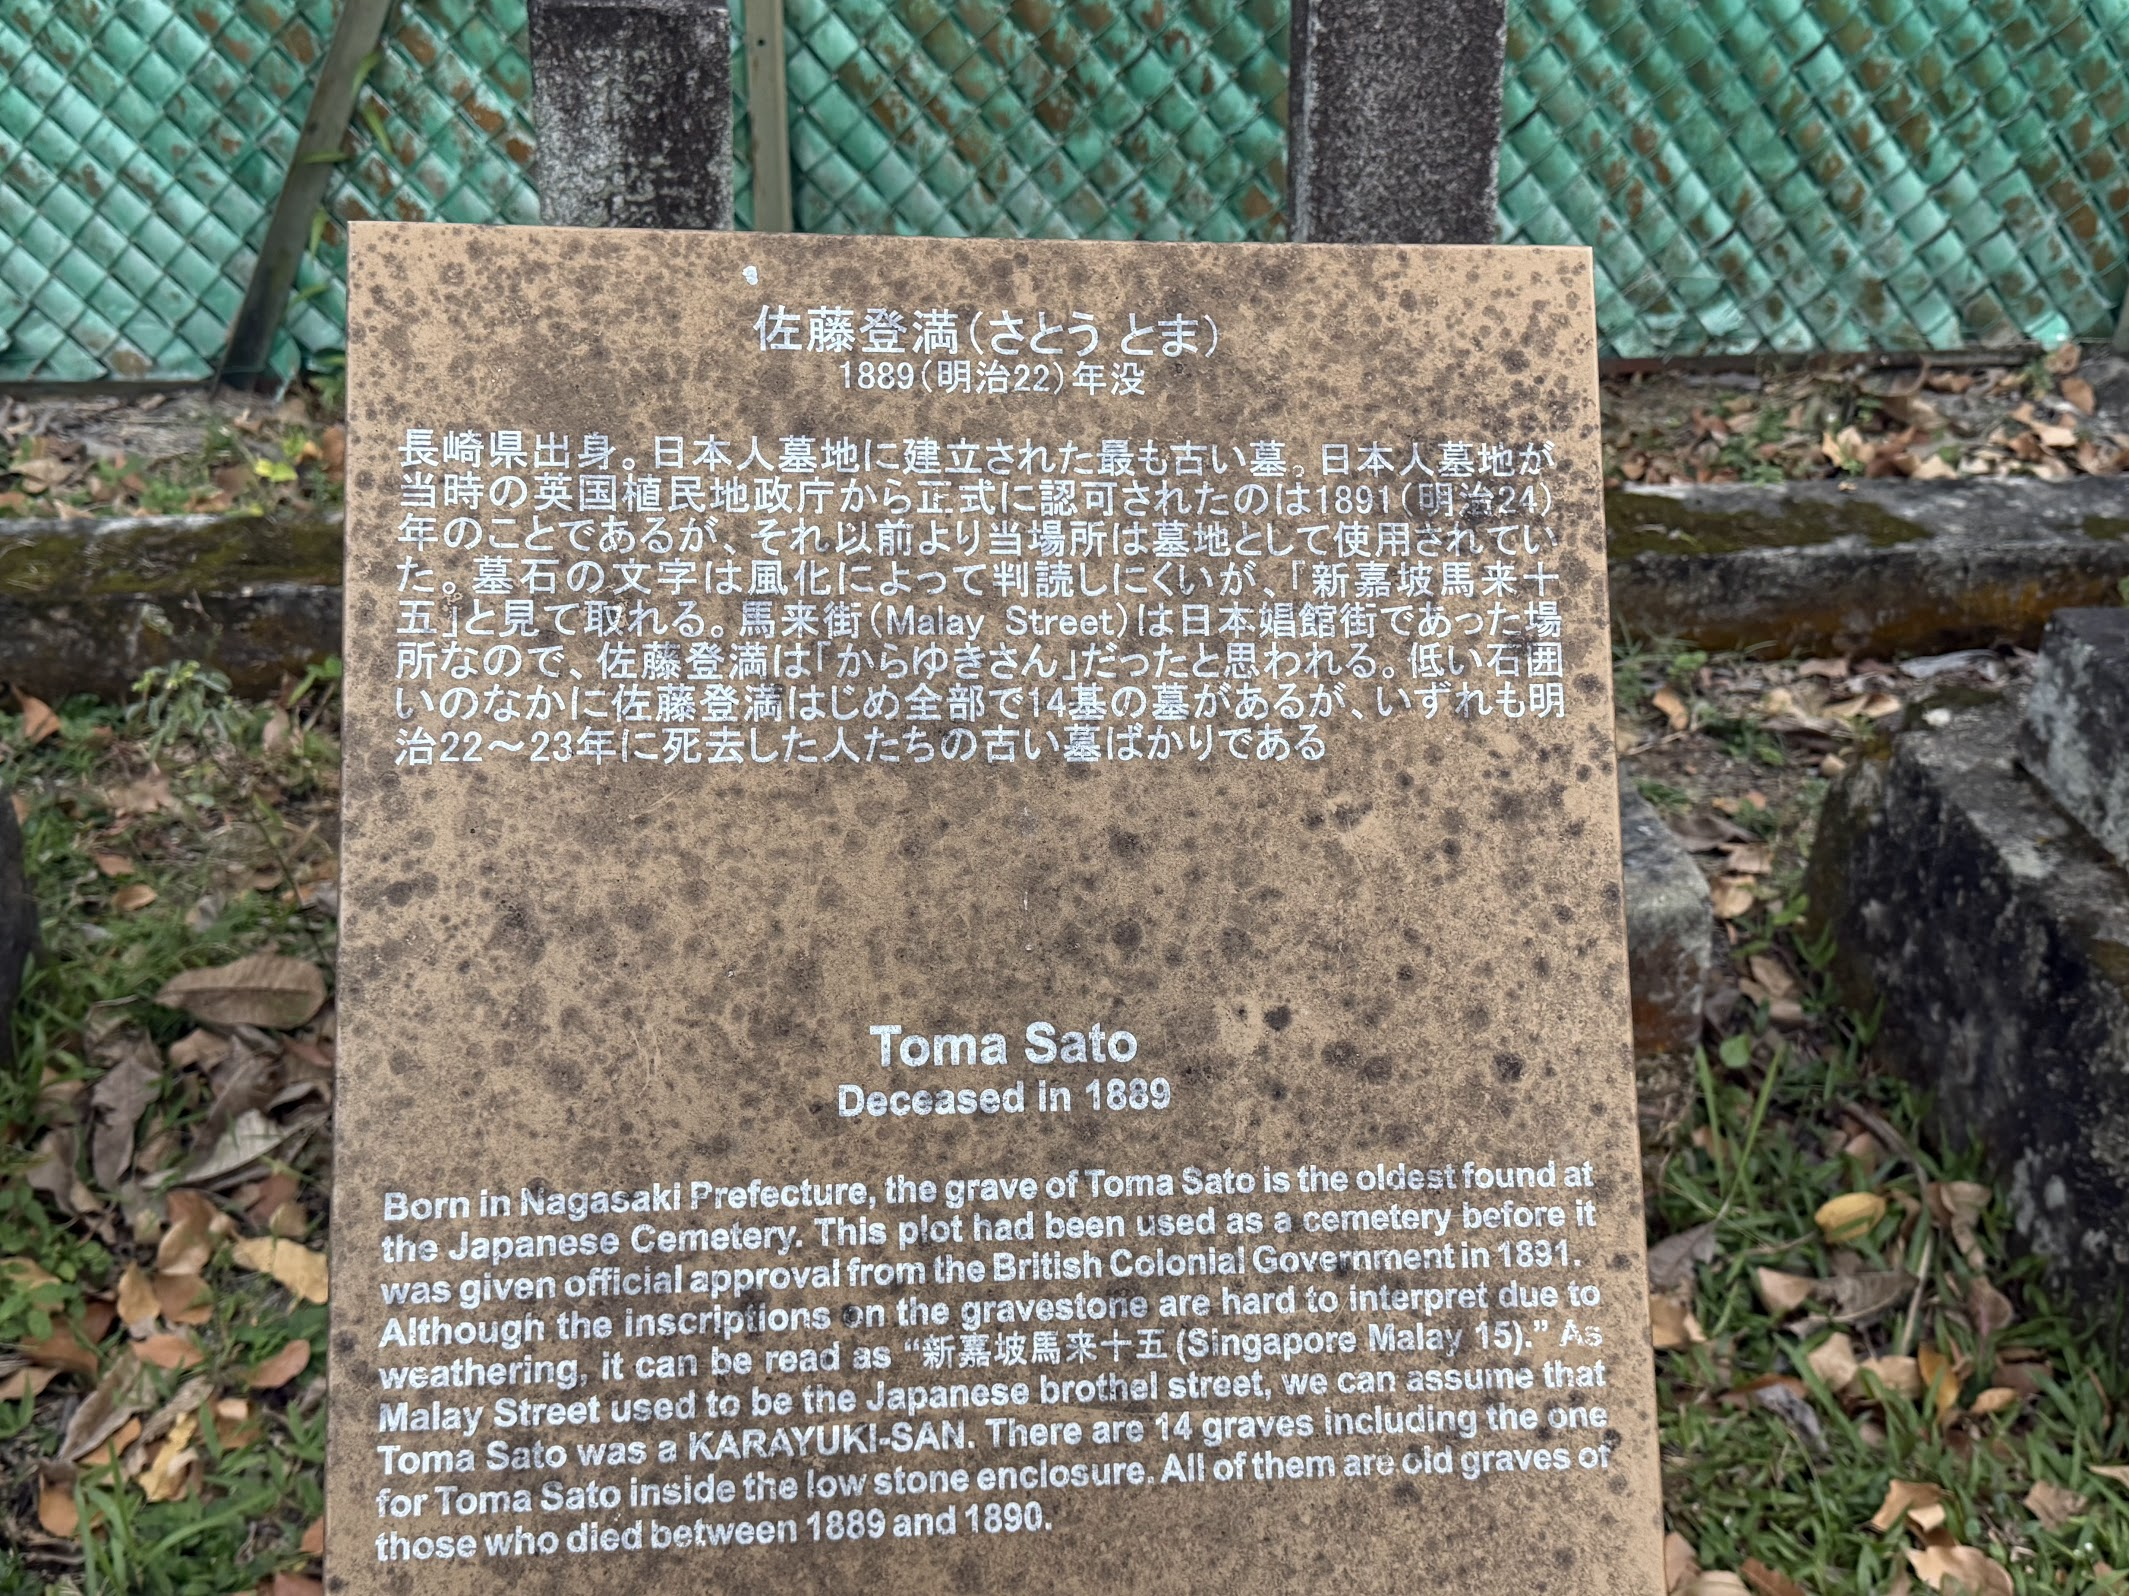
\includegraphics[width=0.8\textwidth]{../../pictures/japanese tomb/IMG_9048}
\caption{Toma Satoと77人の唐行きさんを紹介するパイオニア墓地の説明板}
\end{figure}

シンガポール当局はここに中英日三か国語で「KARAYUKI-SAN」と正式に表記した説明板を設置した。それ自体がすでに歴史の承認だ。しかし、承認の後には何があるのか。

\section{それでも誰かが覚えている}

別の場所に、比較的保存状態の良い日本式の石碑が一基、独立して立っている。碑面には日本語の文字が刻まれ、碑前には香炉と供物台が置かれている。灰はまだ新しく、つい最近誰かが来た証だ。

忘れ去られた墓の多いこの墓地で、この石碑はひときわ貴重に感じられる。誰かが覚えている。子孫なのか、あるいはこの歴史を静かに守り続けている誰かなのか。

\begin{figure}[h]
\centering
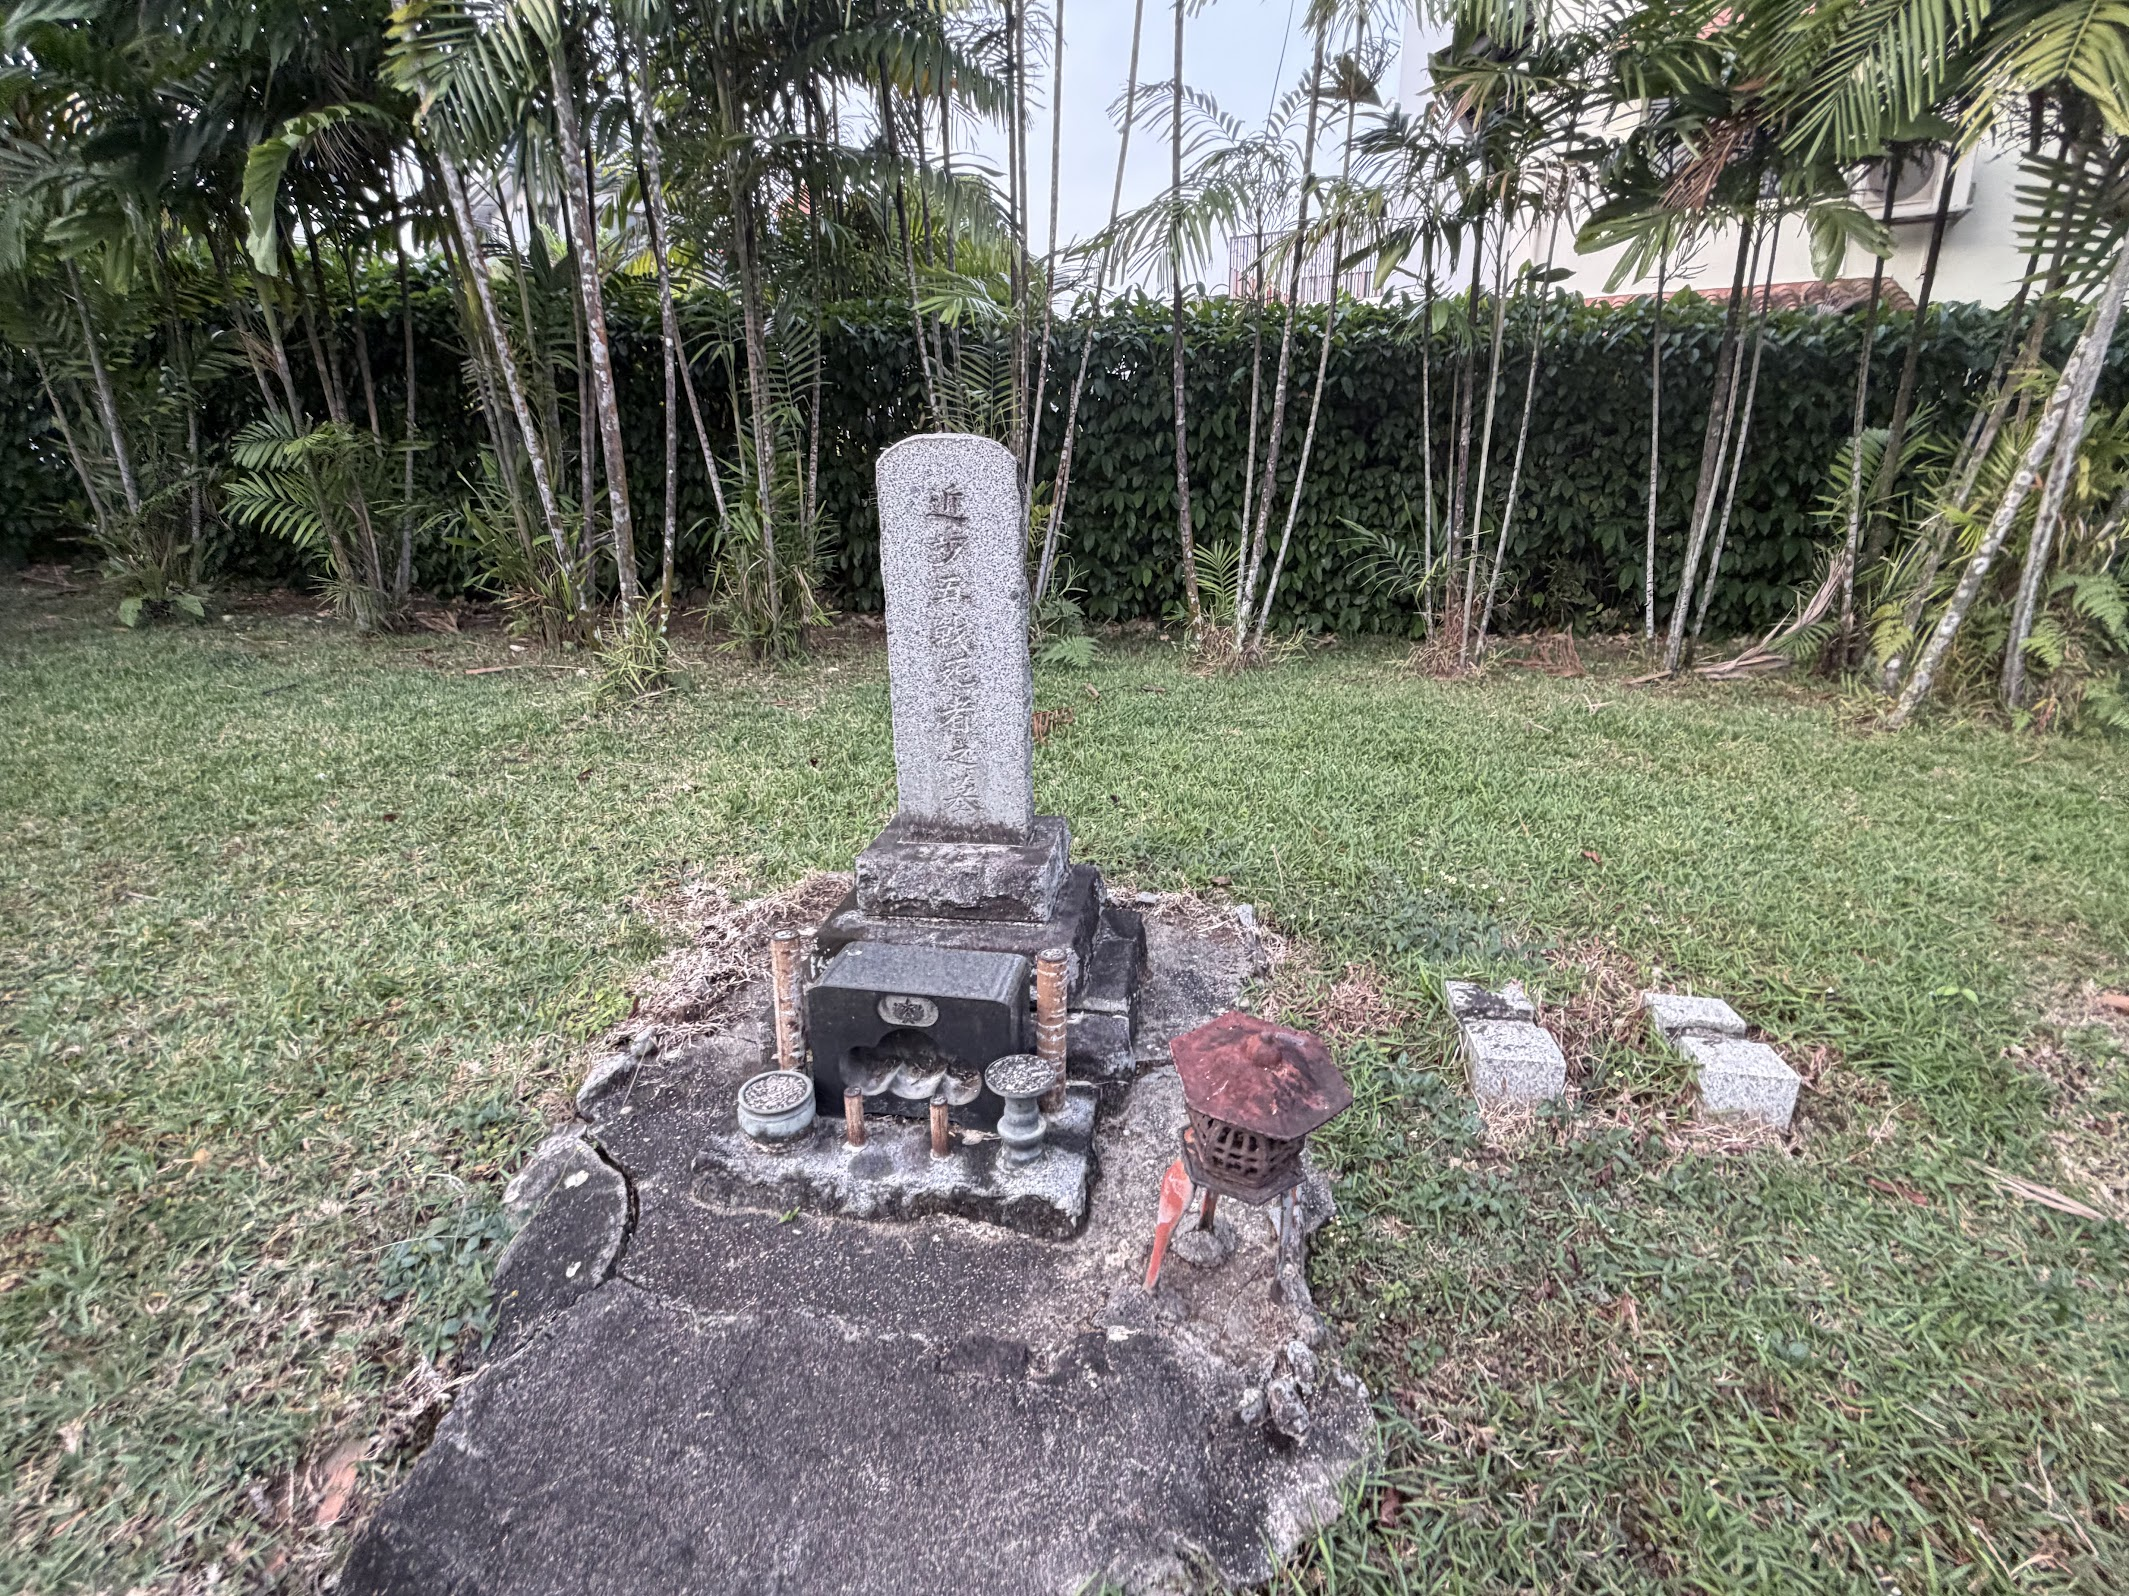
\includegraphics[width=0.8\textwidth]{../../pictures/japanese tomb/IMG_9124}
\caption{香炉と供物が供えられた、今も手入れされている墓碑}
\end{figure}

墓地の反対側には石のベンチが並び、石畳の小道が曲がりくねって続く。ここの雰囲気は、もはや完全に墓地とは言えず、むしろ公園のようだ。シンガポールがこの土地に与えた位置づけは二重だ――追悼の地であり、市民が憩う公共の緑地でもある。

\begin{figure}[h]
\centering
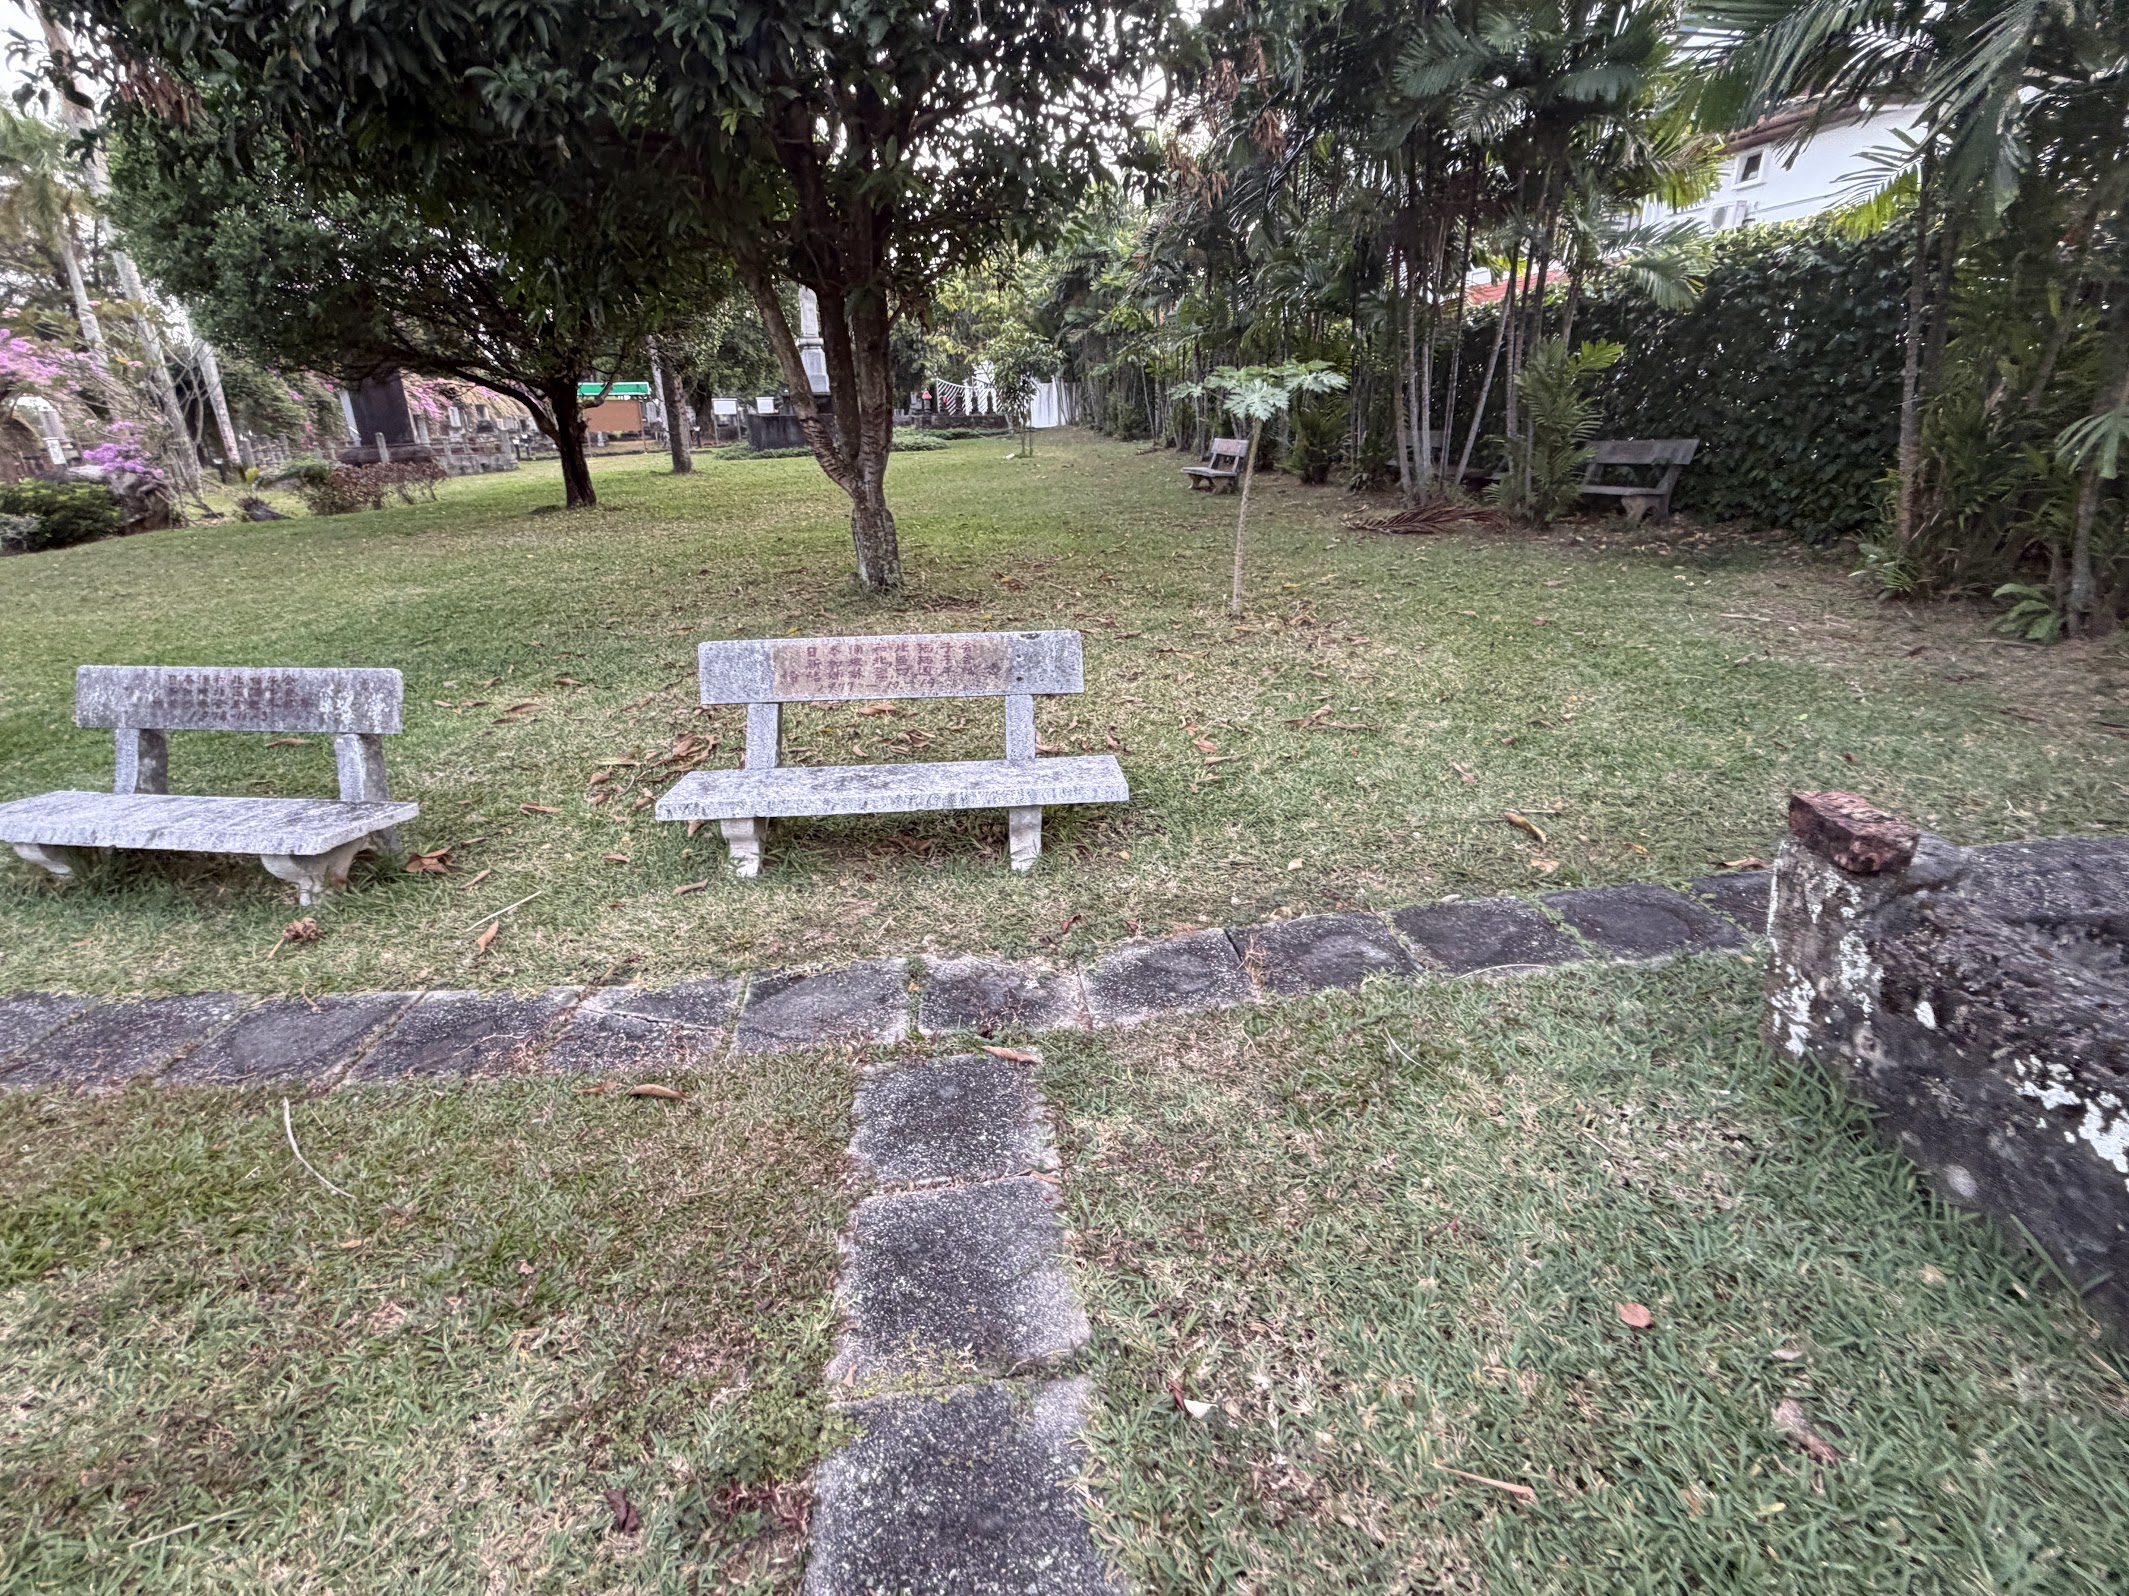
\includegraphics[width=0.8\textwidth]{../../pictures/japanese tomb/IMG_9129}
\caption{石のベンチと曲がりくねった小道――公園のような雰囲気}
\end{figure}

この二重性は沈思を促す。公園化という処理は包容なのか、それとも穏やかな忘却なのか。

\section{クランジ：別の記憶の仕方}

日本人墓地公園の荒廃した静寂とは対照的に、クランジ戦争記念公園はまったく別世界だ。

クランジ戦争墓地（Kranji War Cemetery）はシンガポール北部、住所は 9 Woodlands Road。シンガポール島の北岸の高台に位置し、柔佛海峡（Straits of Johore）を見下ろし、水の向こうにマレーシアを望む。この立地は偶然ではない――1942年2月8日、日本軍はまさにこの海峡を渡り、クランジ川の河口付近に上陸した。今日の墓地から3キロも離れていない場所だ。

この攻勢を率いたのは日本陸軍第25軍司令官・山下奉文（やましたともゆき）大将だった。シンガポールを攻める前に、彼の軍はマレー半島を南下し、馬の代わりに自転車を使って、ジャングルと道路を走り抜け、タイ南部からシンガポール北岸まで約70日で到達した。この「自転車電撃戦（Bicycle Blitzkrieg）」はイギリス軍を完全に不意打ちし、山下は「\textbf{マレーの虎}（Tiger of Malaya）」の異名を得た。イギリス軍の重砲は南の海に向けられており、海から来る敵に備えていた――まさか敵が自転車で背後から来るとは思いもしなかったのだ。

墓地は英連邦戦争墓地委員会（Commonwealth War Graves Commission、CWGC）によって維持管理され、常に清潔に保たれている。白い墓碑が整然と並び、芝生は精緻に刈り込まれ、荘厳で節制された雰囲気だ。ここに眠るのは、1942年のシンガポール陥落（Fall of Singapore）で犠牲になった連合軍兵士たち――イギリス、オーストラリア、インド、マラヤなどの軍人、そして日本軍の侵攻に抵抗して命を落とした人々だ。

すべての墓碑には名前、階級、日付が刻まれている。名無しの墓は一つもない。

この記憶の仕方は、組織的で、資金がある。勝者の記憶は、敗者の記憶よりも長続きし、より整然としている傾向がある。

\section{誰が記憶され、誰が忘れられるのか}

この二つの墓地の間に立ちながら、私は同じ問いを繰り返していた――誰が記憶され、誰が忘れられるのか。

クランジの兵士たちには、名前があり、国籍があり、草を刈り、墓碑を立て、記録を維持する委員会がある。一方、日本人墓地の77人の唐行きさんたちは、歴史上ほぼ完全に無名だった――一枚の説明板が現れて初めて、その存在が通りがかりの人の目に触れるようになった。

彼女たちは戦士でも英雄でもなかった。自国においても恥辱に包まれた存在だった。しかし彼女たちも同じくこの島で死に、同じく熱帯の土に受け入れられた。

今日のシンガポールと日本は友好的な関係にあり、経済的な往来も密接だ。この戦争の歴史は、大々的に清算されることもなく、完全に消し去られることもなかった。日本人墓地は今もあり、説明板も今もある。これがシンガポールの歴史との向き合い方かもしれない――保存するが拡大しない、承認するが固執しない。

刃の上で生き残る小国には、憎しみにかける余裕はあまりない。
